\subsection{\hl{HCMNet 数据集}}

% {A,B,C,D}{S,H,V}{M,H,L}{Ze,On,Tw,Th}
% {Network}{View}{Quartile}{Hourglass}
\renewcommand{\captiontitle}{网络性能评估}
\begin{sidewaystable*}
\begin{center}
\begin{tabular}{ccccccc} \hline
\toprule
名称      & View   & \UNet{} 0                 & \UNet{} 1                 & \UNet{} 2                 & \UNet{} 3                 \\
\midrule
网络 A & All    & $\AAMZe~[\AALZe,~\AAHZe]$ & --                        & --                        & --                        \\
          & \SA{}  & $\ASMZe~[\ASLZe,~\ASHZe]$ & --                        & --                        & --                        \\
          & \HLA{} & $\AHMZe~[\AHLZe,~\AHHZe]$ & --                        & --                        & --                        \\
          & \VLA{} & $\AVMZe~[\AVLZe,~\AVHZe]$ & --                        & --                        & --                        \\
\midrule
网络 B & All    & $\BAMZe~[\BALZe,~\BAHZe]$ & $\BAMOn~[\BALOn,~\BAHOn]$ & --                        & --                        \\
          & \SA{}  & $\BSMZe~[\BSLZe,~\BSHZe]$ & $\BSMOn~[\BSLOn,~\BSHOn]$ & --                        & --                        \\
          & \HLA{} & $\BHMZe~[\BHLZe,~\BHHZe]$ & $\BHMOn~[\BHLOn,~\BHHOn]$ & --                        & --                        \\
          & \VLA{} & $\BVMZe~[\BVLZe,~\BVHZe]$ & $\BVMOn~[\BVLOn,~\BVHOn]$ & --                        & --                        \\
\midrule
网络 C & All    & $\CAMZe~[\CALZe,~\CAHZe]$ & $\CAMOn~[\CALOn,~\CAHOn]$ & $\CAMTw~[\CALTw,~\CAHTw]$ & --                        \\
          & \SA{}  & $\CSMZe~[\CSLZe,~\CSHZe]$ & $\CSMOn~[\CSLOn,~\CSHOn]$ & $\CSMTw~[\CSLTw,~\CSHTw]$ & --                        \\
          & \HLA{} & $\CHMZe~[\CHLZe,~\CHHZe]$ & $\CHMOn~[\CHLOn,~\CHHOn]$ & $\CHMTw~[\CHLTw,~\CHHTw]$ & --                        \\
          & \VLA{} & $\CVMZe~[\CVLZe,~\CVHZe]$ & $\CVMOn~[\CVLOn,~\CVHOn]$ & $\CVMTw~[\CVLTw,~\CVHTw]$ & --                        \\
\midrule
网络 D & All    & $\DAMZe~[\DALZe,~\DAHZe]$ & $\DAMOn~[\DALOn,~\DAHOn]$ & $\DAMTw~[\DALTw,~\DAHTw]$ & $\DAMTh~[\DALTh,~\DAHTh]$ \\
          & \SA{}  & $\DSMZe~[\DSLZe,~\DSHZe]$ & $\DSMOn~[\DSLOn,~\DSHOn]$ & $\DSMTw~[\DSLTw,~\DSHTw]$ & $\DSMTh~[\DSLTh,~\DSHTh]$ \\
          & \HLA{} & $\DHMZe~[\DHLZe,~\DHHZe]$ & $\DHMOn~[\DHLOn,~\DHHOn]$ & $\DHMTw~[\DHLTw,~\DHHTw]$ & $\DHMTh~[\DHLTh,~\DHHTh]$ \\
          & \VLA{} & $\DVMZe~[\DVLZe,~\DVHZe]$ & $\DVMOn~[\DVLOn,~\DVHOn]$ & $\DVMTw~[\DVLTw,~\DVHTw]$ & $\DVMTh~[\DVLTh,~\DVHTh]$ \\
\bottomrule
\end{tabular}
\caption[\captiontitle{}]{\captiontitle{}.
\hl{
表中列出了所有的切面以及所有网络的加权的前景 \IoU{},并给出了四分位数范围的中值.
}
\SA{} 切面的网络性能变现最佳,\HLA{} 切面最差,但是他们的差异并不大.
}
\label{tab:architectureaccuracy}
\end{center}
\end{sidewaystable*}


\subsubsection{\hl{分割}}

我们分别计算了每一幅图的加权的前景 \IoU{},并给出所有预测值的中值和 \IQR{} 值.
详细的结果可以参见表 \ref{tab:architectureaccuracy}.

\renewcommand{\captiontitle}{各个网络加权的前景 \IoU{} 和网络深度关系}
\begin{figure}
\begin{center}
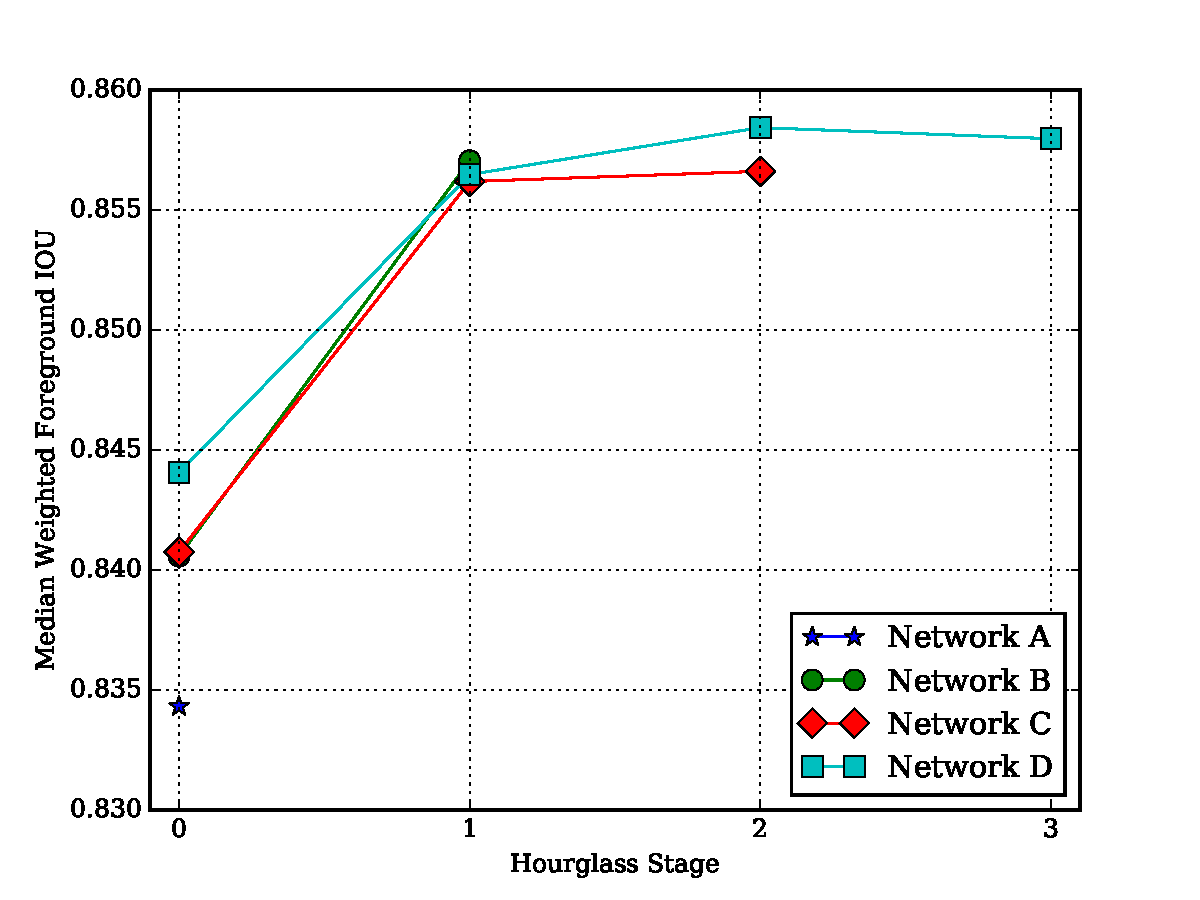
\includegraphics[width=0.5\textwidth]{./data/trendline.pdf}
\caption[\captiontitle]{\captiontitle{}.}
\label{fig:hourglass-accuracy}
\end{center}
\end{figure}


我们对每一个 \UNet{} 中间层的性能也进行了评估,详细内容见图 \ref{fig:hourglass-accuracy}.

\begin{itemize}
\item 虽然网络 A 的参数量最多,但是添加细分割模块可以在粗分割的基础上有效的提升网络性能;
即,网络 B 和 C 的粗分割模块的性能提升了 $\approx~0.007$,网络 D 的粗分割模块也比网络 B 和 C 性能提升了 $\approx~0.003$.
\item 粗分割和细分割之间也有明显的性能提升,即 \UNet{}s 0 和 1(网络 B、C 和 D 分别提升了 $\approx~0.016$, $\approx~0.015$, and $\approx~0.012$).
\item 在网络 C 和 D 中,没有观察到细分割模块中前后的 \UNet{}s 有显著的性能提升.
\end{itemize}

\renewcommand{\captiontitle}{每一切面和类别的 \IoU{} 直方图}
\begin{figure*}
\begin{center}
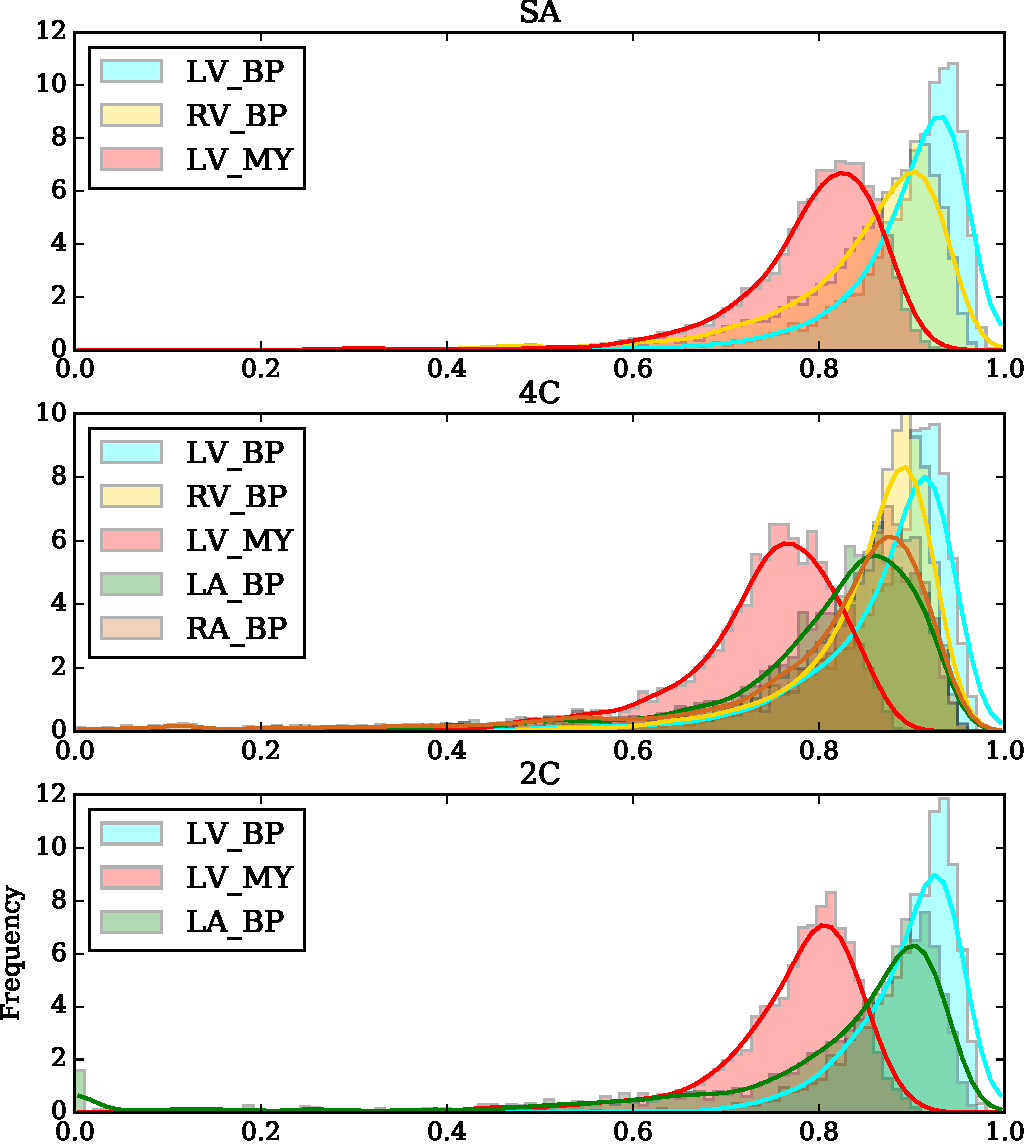
\includegraphics[width=1.0\textwidth]{./data/histograms.pdf}
\caption[\captiontitle]{\captiontitle{}. \SA{} 切面的结果最佳,\HLA{} 切面的结果最差,但是差异不大.\\
\hl{
LV\_BP:左室血池; RV\_BP:右室血池;LV\_MY:左室心肌;LA\_BP左房血池;右房血池.}
}
\label{fig:histograms}
\end{center}
\end{figure*}


考虑到不同解剖结构的分割性能会有所区别,我们将表现最好的网络 (\bestnetwork{})的每个图的的每个结构结构和每个临床切面的 \IoU{} 直方图绘制了出来,如图 \ref{fig:histograms} 所示.
在这所有的临床切面中,性能最差的是左室心肌,最好的是左室血池,其他的结构的在中等水平.
从直观上来看,相对较差的左室心肌分割性能在与边界结构的分割错误.
因此,那些有着较高的周长与面积之比的结构(如左室心肌,有着内部和外部两部分周长,也就是心内膜和心外膜)分割结果就比较差.
而左室血池的分割性能较好则有以下几个可能的因素.

\begin{itemize}
\item 左室血池周长上有高对比度的左室心肌边界.
\item 相比于其他心脏结构结构,不同被试者的左室血池差异较小.
\item 本研究使用的三个正交平面都是相对于左室来定义的;因此,不同被试者之间的左室差异也比较小.
\end{itemize}

\hl{
图 \ref{fig:roc} 为 PR 曲线,其中纵轴为成功率,成功率定义为 \IoU{} 大于阈值 $0.4$ 到 $1.0$ 的被试者百分比.
PR 曲线下面积(AUR)表示 \omeganet{} 网络的准确度.
我们还计算了失败率,即 $1 - \mathrm{success rate}$.
例如,保守估计一个 \IoU{} $< 0.9$ 时对应的失败率大约为 $1\%$.
}

\bestnetwork{} 在所有切面的正常受试者以及 \HCM{} 受试者的分割结果如图 \ref{fig:representative-results-control} 和 \ref{fig:representative-results-overt} 所示.
注意一下,分割真实值也是经过预测的参数进行了变换,这样子才能对中间帧进行插值.
网络成功地将这些例图都变换到了一个典型方向.
并且需要说明的是,心肌分割均除去了乳头肌和小梁.
而且,网络都很好的识别出了长轴图的房室瓣,这一点在以后的工作中很值得注意.

\renewcommand{\captiontitle}{PR 曲线}
\begin{figure}
\begin{center}
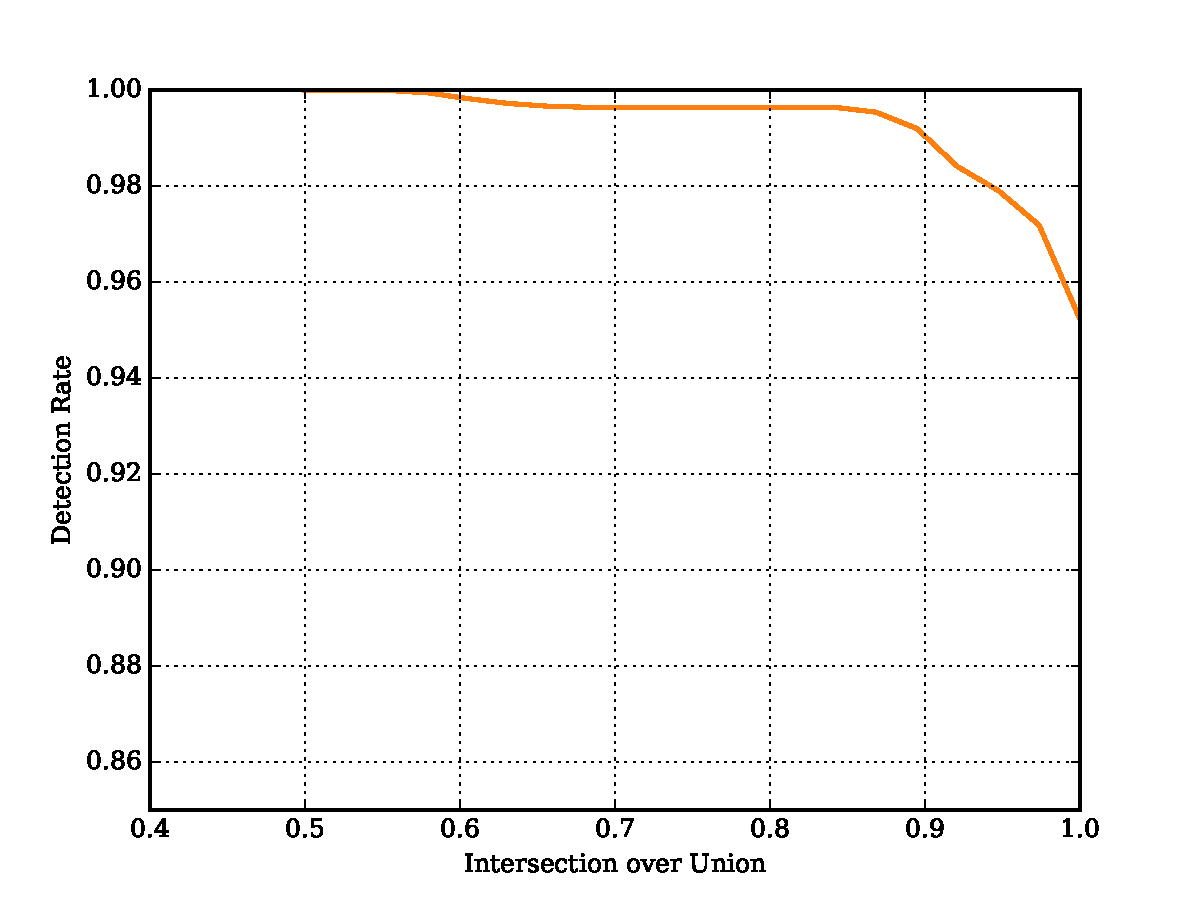
\includegraphics[width=0.5\textwidth]{./data/det_ROC_hgd_3.pdf}
\caption[\captiontitle]{\captiontitle{}.
}
\label{fig:roc}
\end{center}
\end{figure}


\renewcommand{\captiontitle}{健康受试者的分割结果}
\begin{figure*}
\begin{center}

\setlength{\tabcolsep}{1pt}

\begin{tabular}{ccccc}

\toprule
\SA{}(底层切片) & \SA{} (中间切片) & \SA{}(顶层切片) & \HLA{} & \VLA{} \\
\midrule

\multicolumn{5}{c}{未对齐方向的原始图像:$\image$} \\

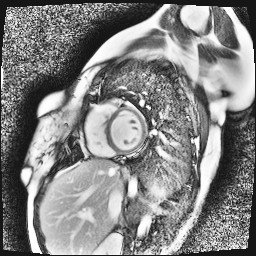
\includegraphics[width=0.19\textwidth]{./data/representative-results/control/HCMNet_2600035/00_SAX/BASE/0.png} &
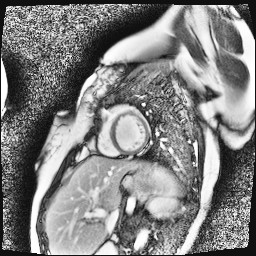
\includegraphics[width=0.19\textwidth]{./data/representative-results/control/HCMNet_2600035/00_SAX/MID/0.png} &
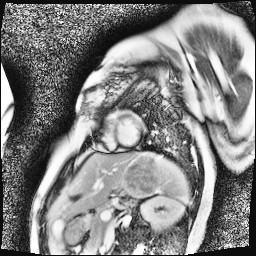
\includegraphics[width=0.19\textwidth]{./data/representative-results/control/HCMNet_2600035/00_SAX/APEX/0.png} &
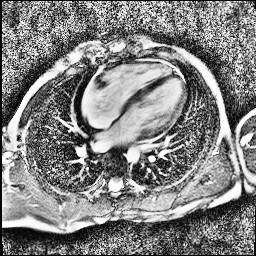
\includegraphics[width=0.19\textwidth]{./data/representative-results/control/HCMNet_1700012/01_HLA/00/0.png} &
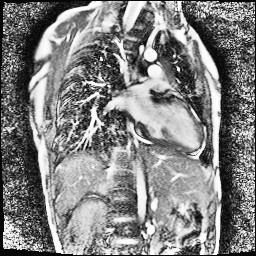
\includegraphics[width=0.19\textwidth]{./data/representative-results/control/HCMNet_1700012/02_VLA/00/0.png} \\

\multicolumn{5}{c}{结构定位} \\

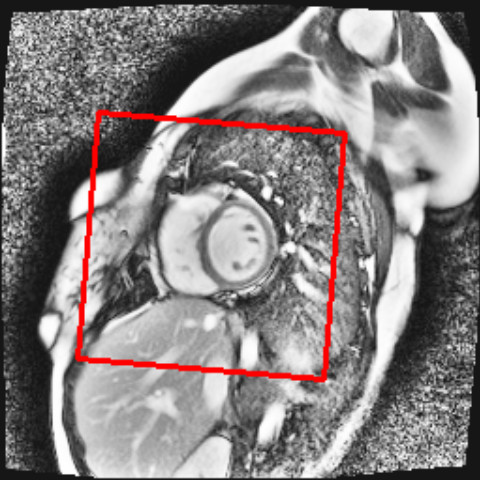
\includegraphics[width=0.19\textwidth]{./data/representative-results/control/HCMNet_2600035/00_SAX/BASE/0_bbox.png} &
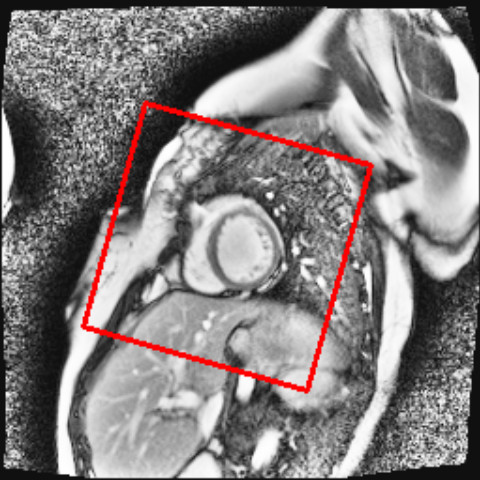
\includegraphics[width=0.19\textwidth]{./data/representative-results/control/HCMNet_2600035/00_SAX/MID/0_bbox.png} &
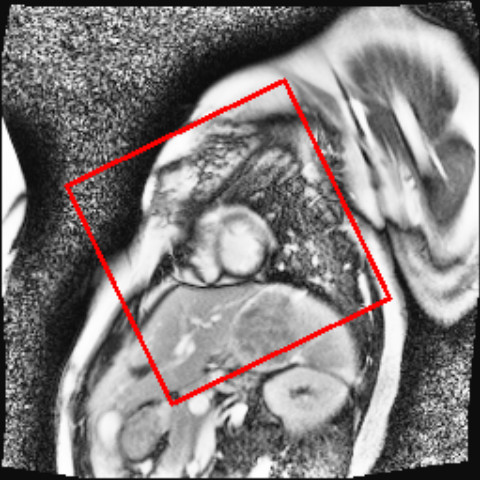
\includegraphics[width=0.19\textwidth]{./data/representative-results/control/HCMNet_2600035/00_SAX/APEX/0_bbox.png} &
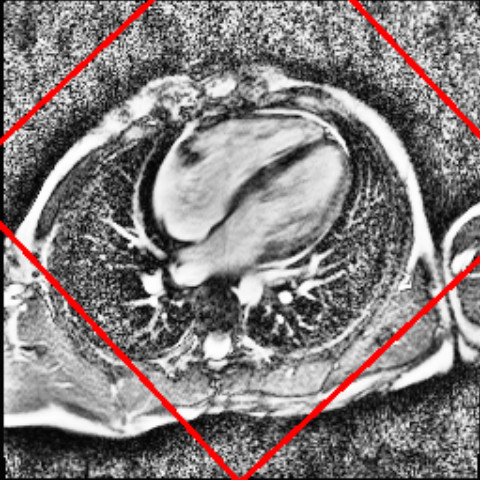
\includegraphics[width=0.19\textwidth]{./data/representative-results/control/HCMNet_1700012/01_HLA/00/0_bbox.png} &
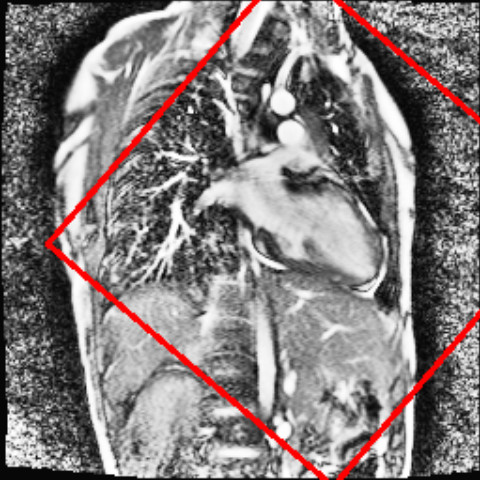
\includegraphics[width=0.19\textwidth]{./data/representative-results/control/HCMNet_1700012/02_VLA/00/0_bbox.png} \\

\multicolumn{5}{c}{在典型方向下的分割预测值:$S^\prime$} \\

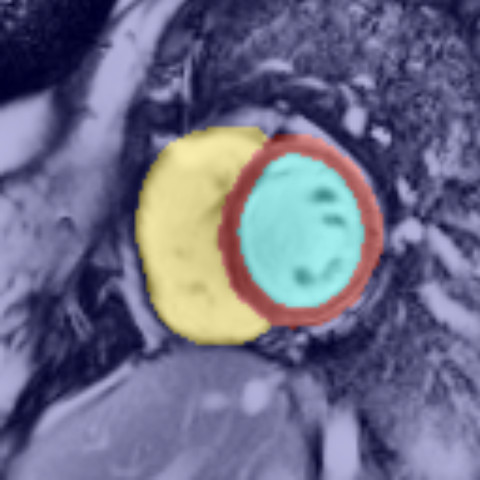
\includegraphics[width=0.19\textwidth]{./data/representative-results/control/HCMNet_2600035/00_SAX/BASE/0_pred.png} &
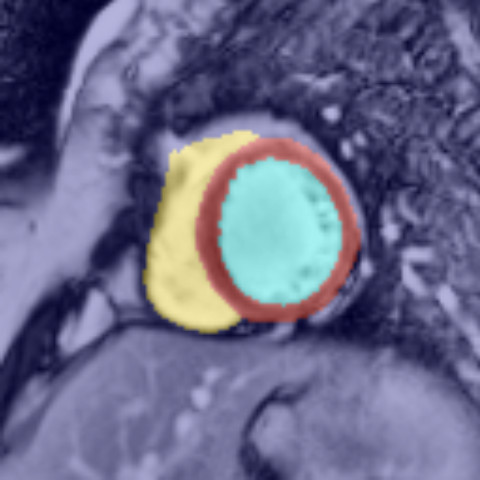
\includegraphics[width=0.19\textwidth]{./data/representative-results/control/HCMNet_2600035/00_SAX/MID/0_pred.png} &
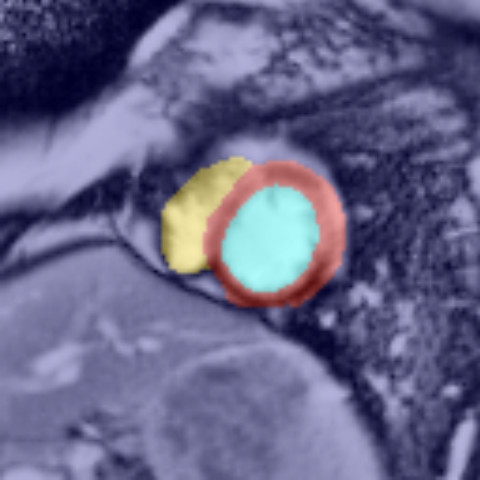
\includegraphics[width=0.19\textwidth]{./data/representative-results/control/HCMNet_2600035/00_SAX/APEX/0_pred.png} &
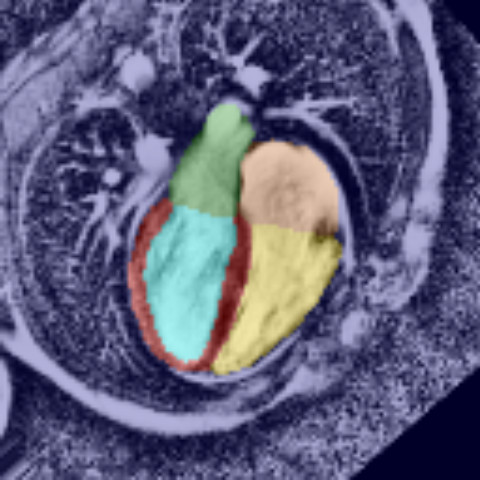
\includegraphics[width=0.19\textwidth]{./data/representative-results/control/HCMNet_1700012/01_HLA/00/0_pred.png} &
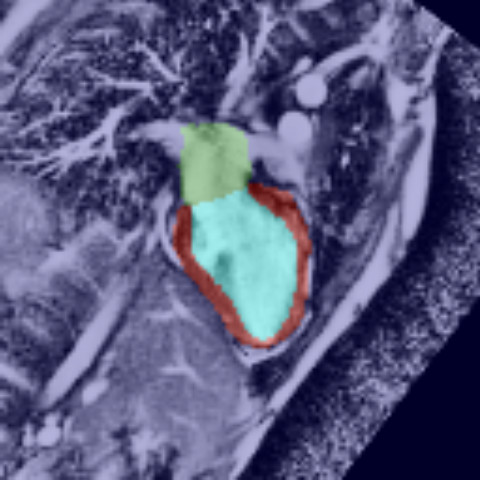
\includegraphics[width=0.19\textwidth]{./data/representative-results/control/HCMNet_1700012/02_VLA/00/0_pred.png} \\
\bottomrule

\multicolumn{5}{c}{在典型方向下的分割真实值:$\hat{S}^\prime$} \\

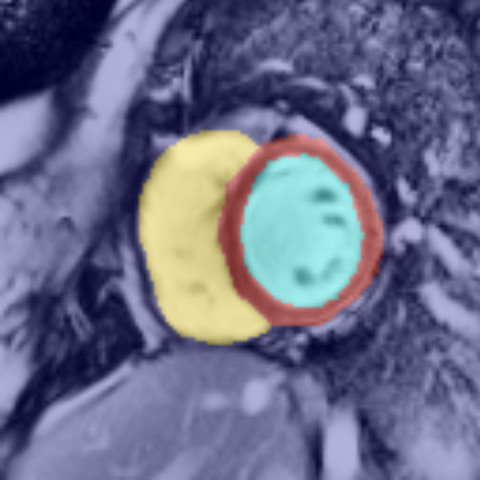
\includegraphics[width=0.19\textwidth]{./data/representative-results/control/HCMNet_2600035/00_SAX/BASE/0_gt.png} &
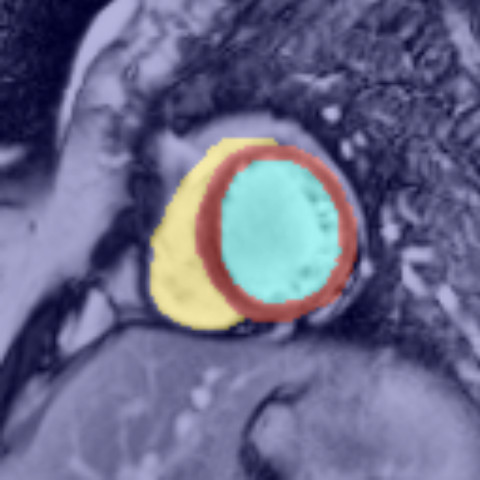
\includegraphics[width=0.19\textwidth]{./data/representative-results/control/HCMNet_2600035/00_SAX/MID/0_gt.png} &
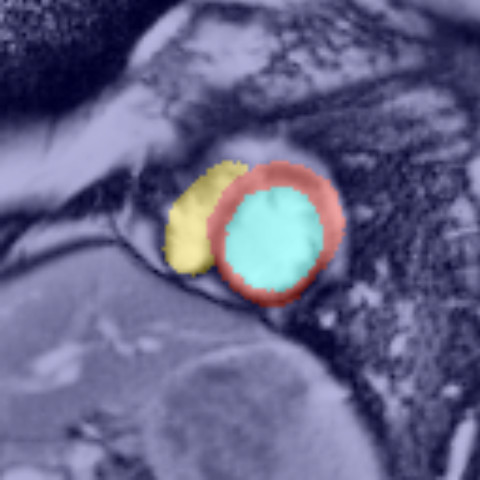
\includegraphics[width=0.19\textwidth]{./data/representative-results/control/HCMNet_2600035/00_SAX/APEX/0_gt.png} &
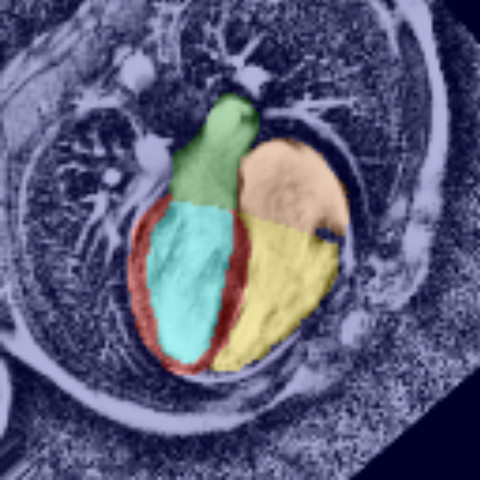
\includegraphics[width=0.19\textwidth]{./data/representative-results/control/HCMNet_1700012/01_HLA/00/0_gt.png} &
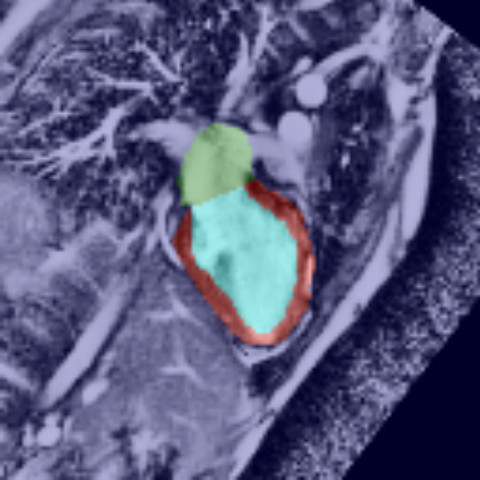
\includegraphics[width=0.19\textwidth]{./data/representative-results/control/HCMNet_1700012/02_VLA/00/0_gt.png} \\
\bottomrule

\end{tabular}

\caption[\captiontitle]{\captiontitle{}. 详细讨论请参考正文内容.}
\label{fig:representative-results-control}
\end{center}
\end{figure*}

\renewcommand{\captiontitle}{患有 \HCM{} 的患者的分割结果}
\begin{figure*}
\begin{center}

\setlength{\tabcolsep}{1pt}

\begin{tabular}{ccccc}

\toprule
\SA{}(底层切片) & \SA{}(中间切片)& \SA{}(顶层切片) & \HLA{} & \VLA{} \\
\midrule

\multicolumn{5}{c}{未对齐方向的原始图像:$\image$} \\

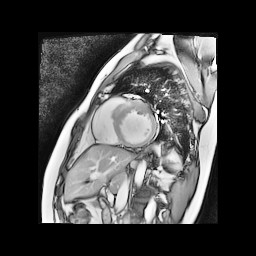
\includegraphics[width=0.19\textwidth]{./data/representative-results/overt/HCMNet_1100083/00_SAX/BASE/0.png} &
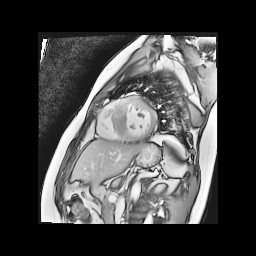
\includegraphics[width=0.19\textwidth]{./data/representative-results/overt/HCMNet_1100083/00_SAX/MID/0.png} &
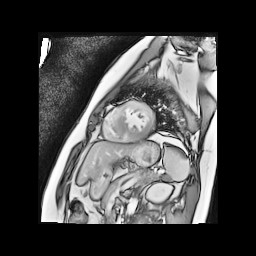
\includegraphics[width=0.19\textwidth]{./data/representative-results/overt/HCMNet_1100083/00_SAX/APEX/0.png} &
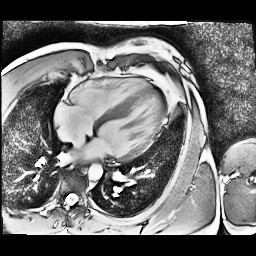
\includegraphics[width=0.19\textwidth]{./data/representative-results/overt/HCMNet_1100367/01_HLA/00/0.png} &
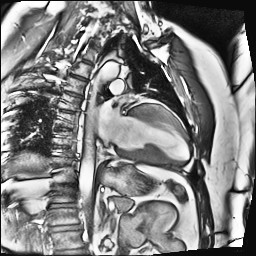
\includegraphics[width=0.19\textwidth]{./data/representative-results/overt/HCMNet_1100027/02_VLA/00/0.png} \\

\multicolumn{5}{c}{结构定位} \\

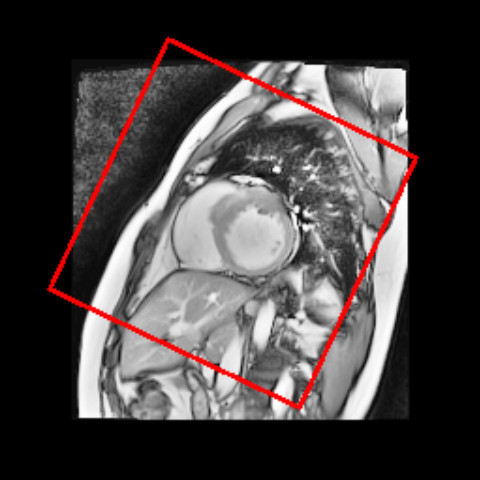
\includegraphics[width=0.19\textwidth]{./data/representative-results/overt/HCMNet_1100083/00_SAX/BASE/0_bbox.png} &
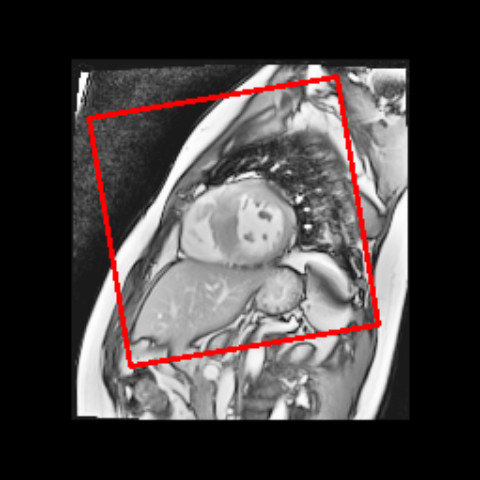
\includegraphics[width=0.19\textwidth]{./data/representative-results/overt/HCMNet_1100083/00_SAX/MID/0_bbox.png} &
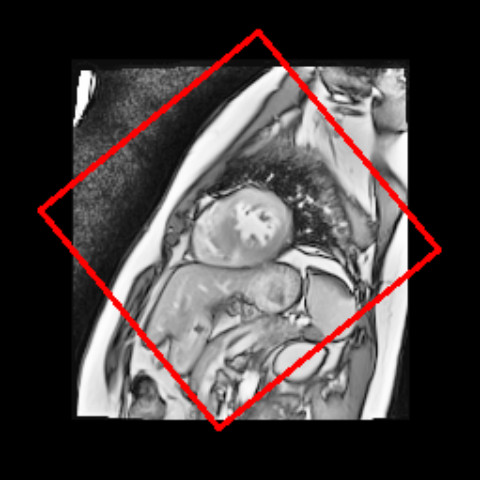
\includegraphics[width=0.19\textwidth]{./data/representative-results/overt/HCMNet_1100083/00_SAX/APEX/0_bbox.png} &
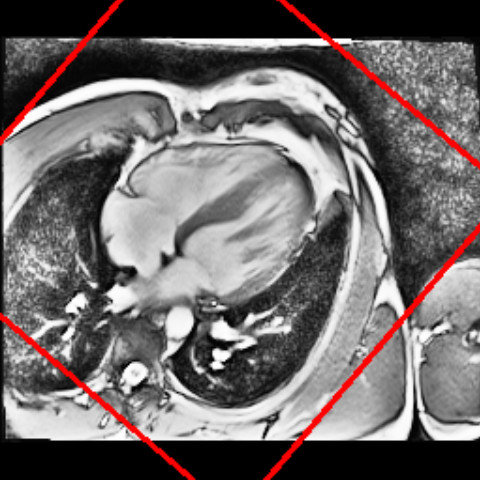
\includegraphics[width=0.19\textwidth]{./data/representative-results/overt/HCMNet_1100367/01_HLA/00/0_bbox.png} &
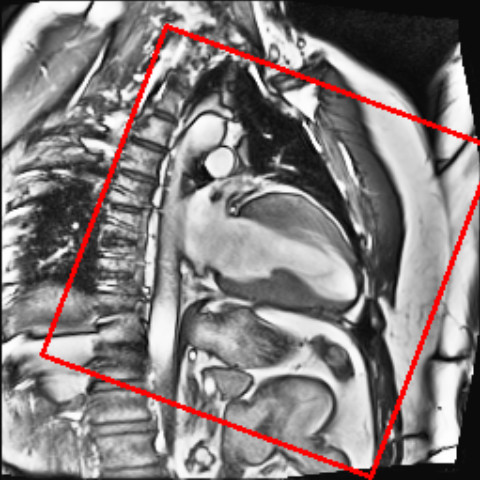
\includegraphics[width=0.19\textwidth]{./data/representative-results/overt/HCMNet_1100027/02_VLA/00/0_bbox.png} \\

\multicolumn{5}{c}{在典型方向下的分割预测值:$S^\prime$} \\

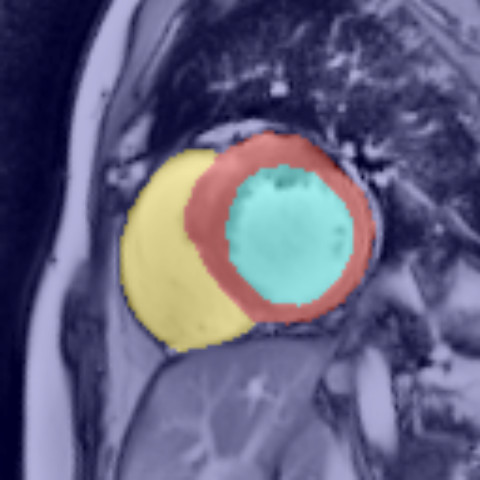
\includegraphics[width=0.19\textwidth]{./data/representative-results/overt/HCMNet_1100083/00_SAX/BASE/0_pred.png} &
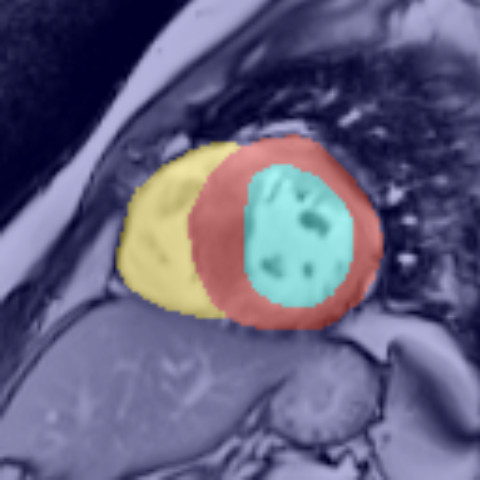
\includegraphics[width=0.19\textwidth]{./data/representative-results/overt/HCMNet_1100083/00_SAX/MID/0_pred.png} &
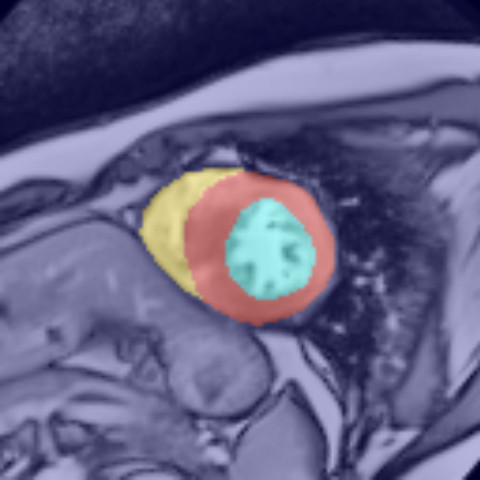
\includegraphics[width=0.19\textwidth]{./data/representative-results/overt/HCMNet_1100083/00_SAX/APEX/0_pred.png} &
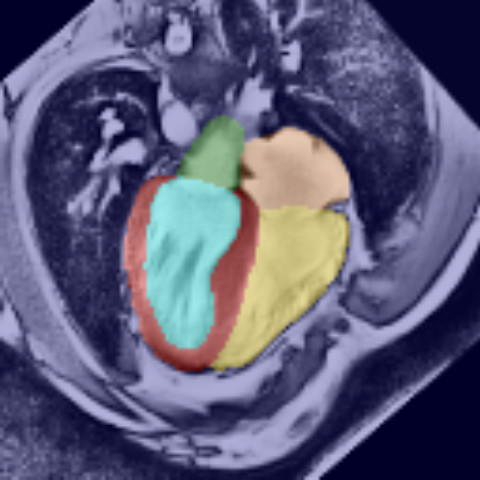
\includegraphics[width=0.19\textwidth]{./data/representative-results/overt/HCMNet_1100367/01_HLA/00/0_pred.png} &
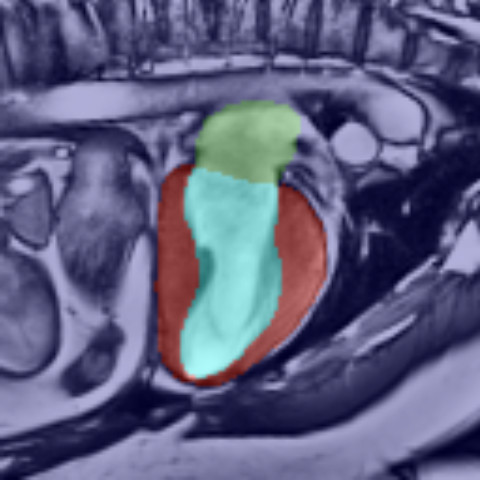
\includegraphics[width=0.19\textwidth]{./data/representative-results/overt/HCMNet_1100027/02_VLA/00/0_pred.png} \\
\bottomrule

\multicolumn{5}{c}{在典型方向下的分割真实值:$\hat{S}^\prime$} \\

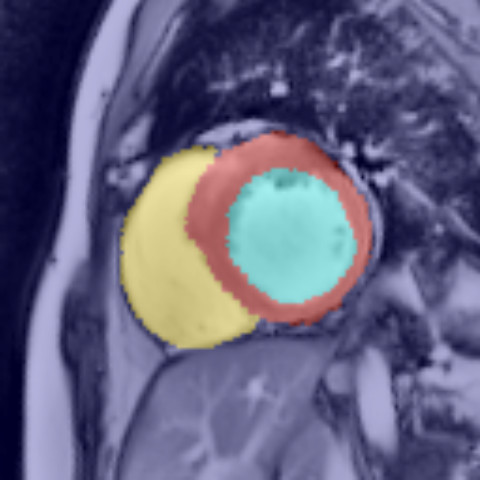
\includegraphics[width=0.19\textwidth]{./data/representative-results/overt/HCMNet_1100083/00_SAX/BASE/0_gt.png} &
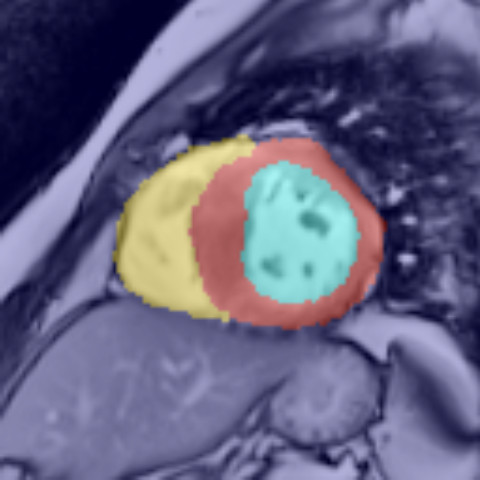
\includegraphics[width=0.19\textwidth]{./data/representative-results/overt/HCMNet_1100083/00_SAX/MID/0_gt.png} &
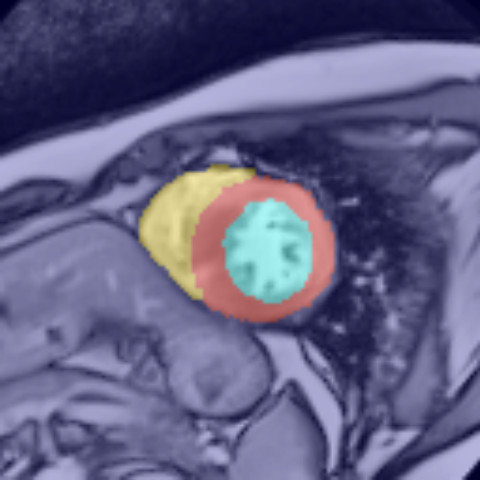
\includegraphics[width=0.19\textwidth]{./data/representative-results/overt/HCMNet_1100083/00_SAX/APEX/0_gt.png} &
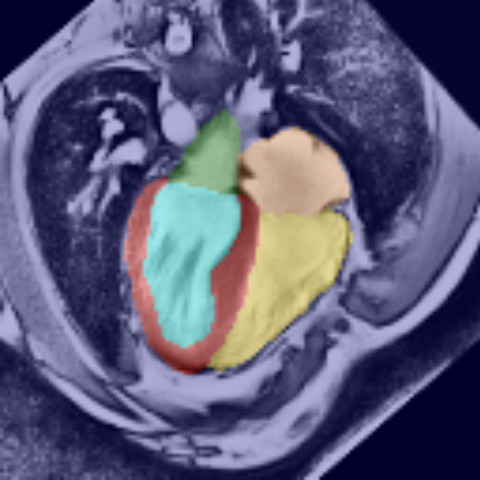
\includegraphics[width=0.19\textwidth]{./data/representative-results/overt/HCMNet_1100367/01_HLA/00/0_gt.png} &
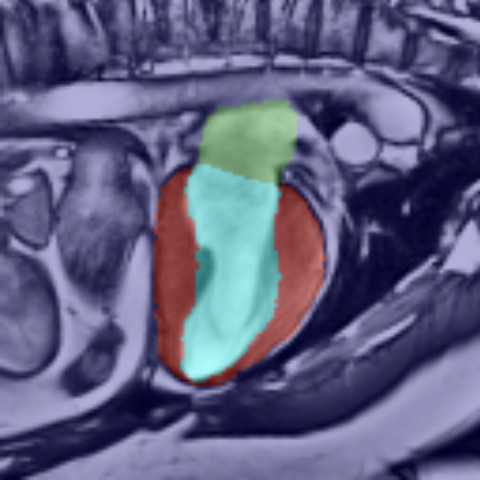
\includegraphics[width=0.19\textwidth]{./data/representative-results/overt/HCMNet_1100027/02_VLA/00/0_gt.png} \\
\bottomrule

\end{tabular}

\caption[\captiontitle]{\captiontitle{}.详细讨论请参考正文内容.}
\label{fig:representative-results-overt}
\end{center}
\end{figure*}


\subsubsection{变换参数}

\renewcommand{\captiontitle}{变换误差}
\begin{sidewaysfigure*}
\begin{center}
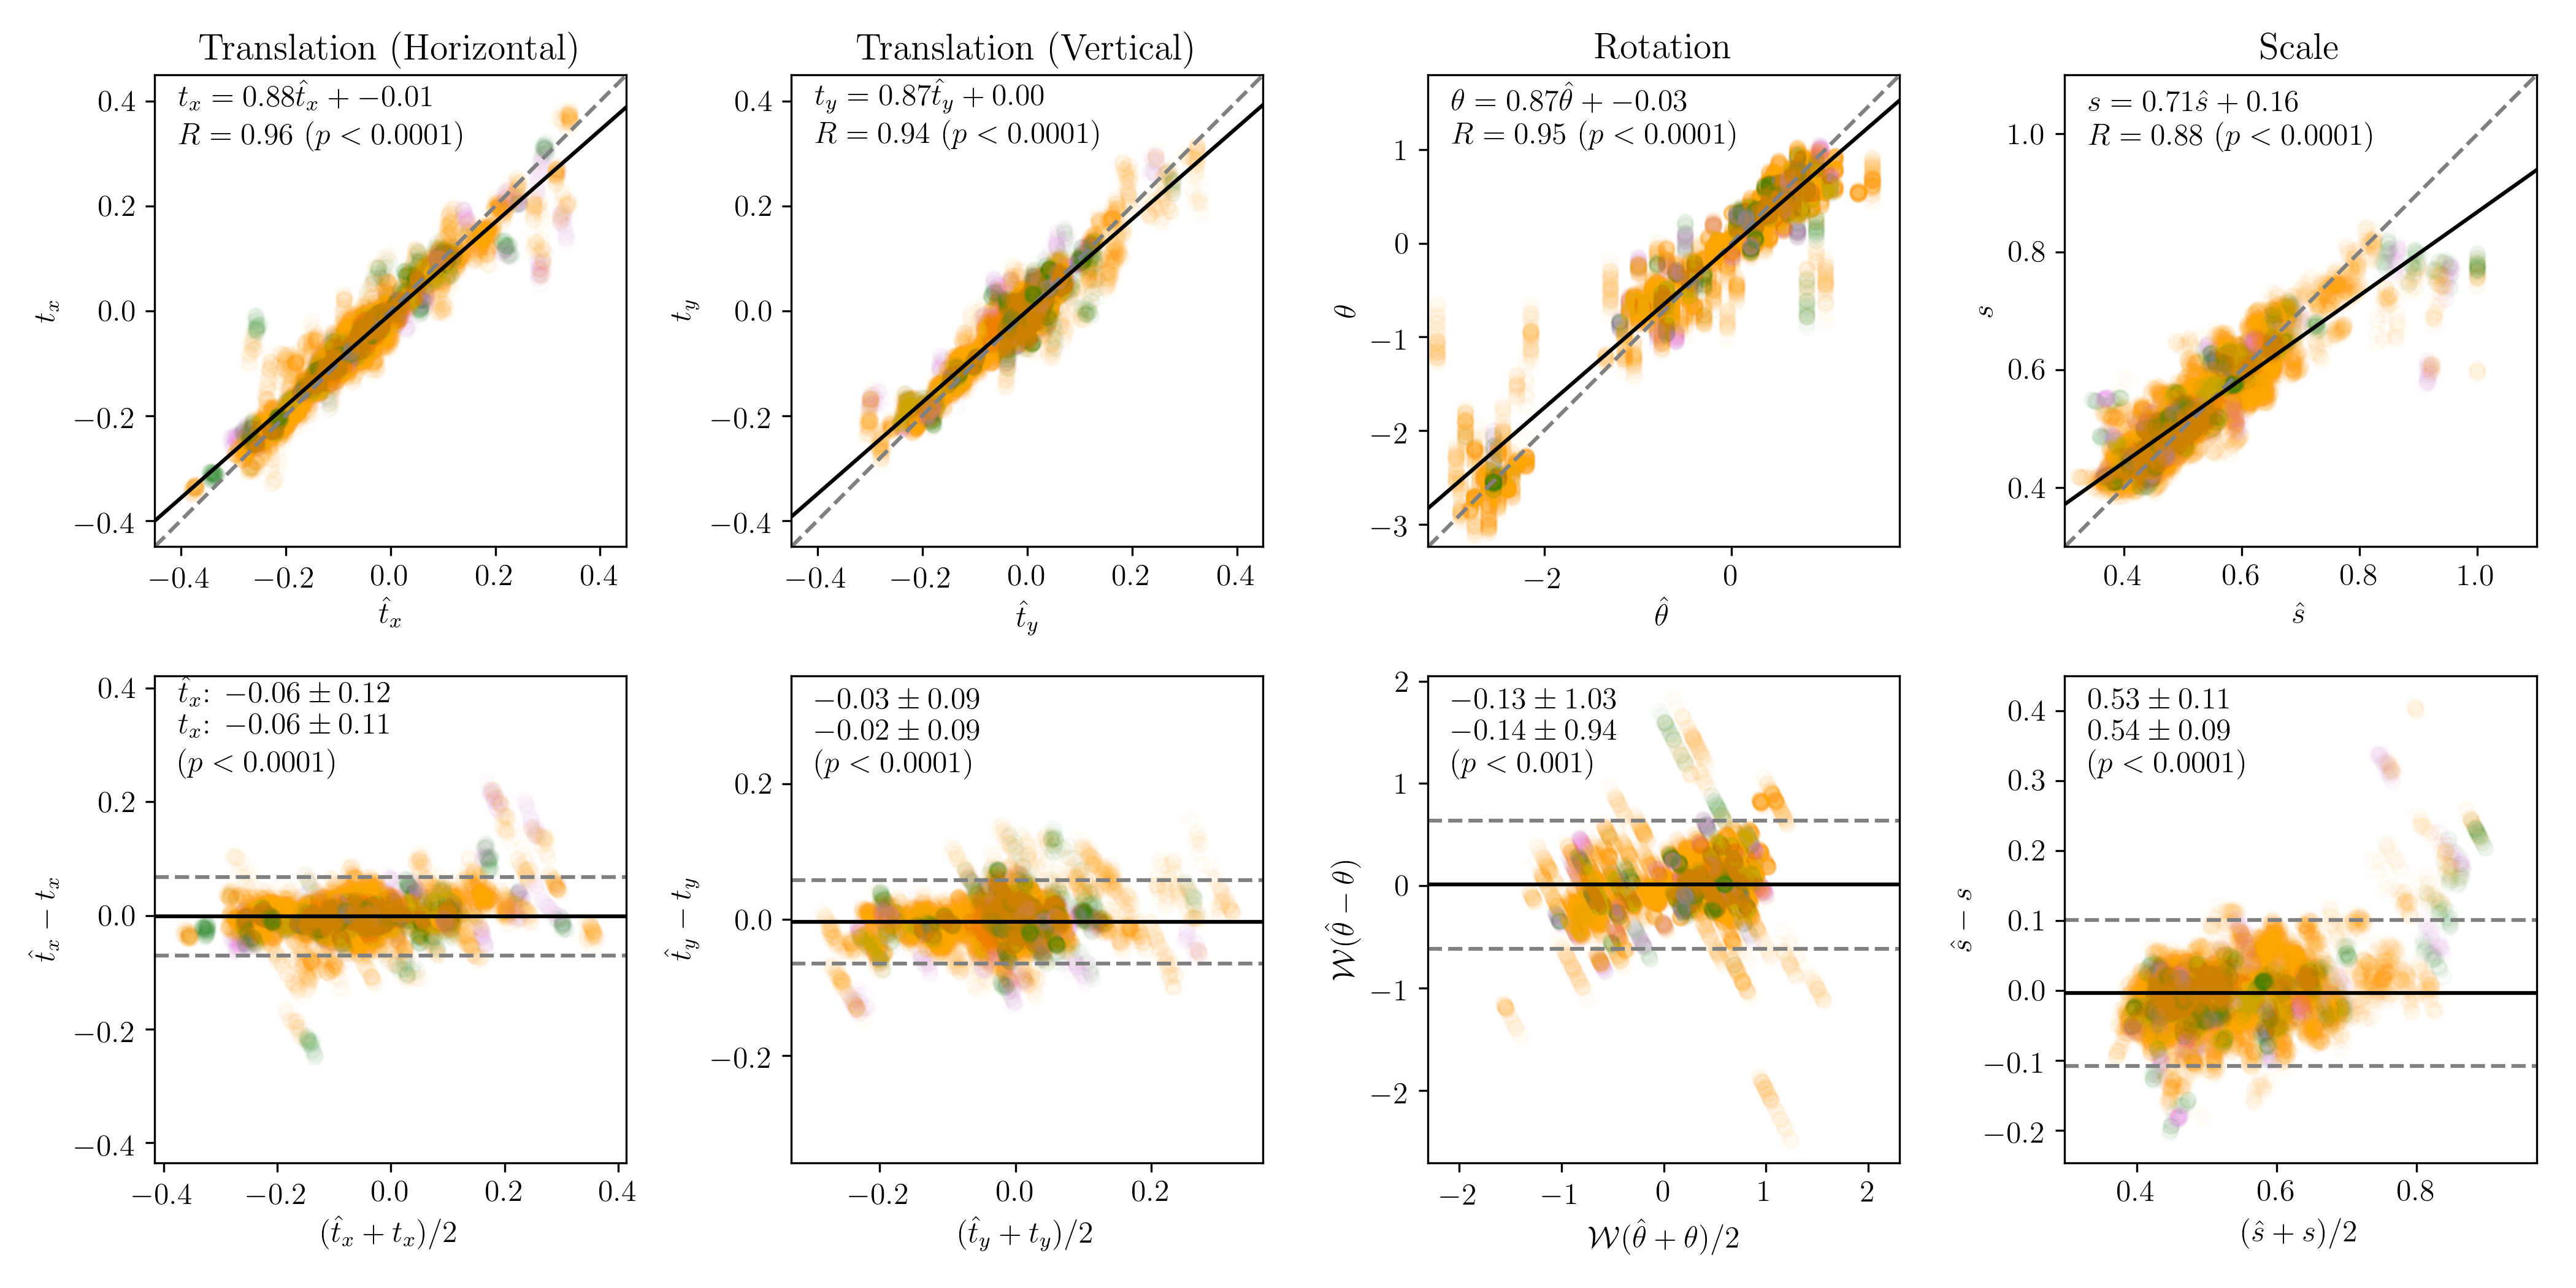
\includegraphics[width=1.0\textwidth]{./data/matrix-loss.png}
\caption[\captiontitle]{\captiontitle{}.
我们给出了变换参数的预测值与真实值之间的相关系数图(上)和 Bland-Altman 图(下).
\SA{}、\HLA{} 和 \VLA{} 误差分贝用橙色、绿色和紫色点表示(所有的点都做了半透明处理,以方便查看).
在相关系数图中,最佳的拟合线用黑色实线表示,理想的线条($y = x$)用灰色的虚线表示.
我们也给出了拟合线的公式和皮尔森相关系数 $R$.
而在 Bland-Altman 图中,误差均值用黑色水平实线表示,$\pm 1.96$ 的标准差界线用灰色水平虚线表示.
}
\label{fig:matrix-loss}
\end{center}
\end{sidewaysfigure*}



我们通过相关系数和 Bland Altman 图(见图 \ref{fig:matrix-loss})来比较参数真实值与性能最好的网络(\bestnetwork{})进行比较.
需要指出的是,变换参数的真实值,特别是旋转和缩放,并不是在所有切面上均匀分布的.
非随机的旋转应该是由以下原因导致的,包括病人与扫描器的相对位置,扫查平面的流程,心脏和胸腔的位置以及不同扫查平面之间的关系都是非随机的;而非随机的缩放则可能是因为在每一切面中结构结构的可视范围不同.

水平平移,垂直平移和旋转参数的预测值与真实值是高度相关的($R \approx~0.95$, $p < 0.0001$),而预测参数相比于真实值都是略有低估了($\approx~0.87$).
从 Bland-Altman 图中看来,系统的偏移并不明显;$95\%$ 的平移误差在 $\pm 0.07$(以归一化后的图像坐标计算)以内,而 $95\%$ 的旋转误差在 $\pm 0.63$ 以内(以弧度计算).
在那些 $5\%$ 的离群值里,大部分都集中在长轴切面(\HLA{} 和 \VLA{}).
考虑到每个病人都提供了三个短轴切面,而只有两个长轴切面,这一点应该不太令人感到惊讶.

比起平移和旋转,缩放的预测值与真实值的相关系数略低,但依然是不错的($R = 0.88$, $p < 0.0001$);缩放的预测值比起真实值依然是低估了($s = 0.71\hat{s} + 0.16$).
注意到在网络大约有个 $\hat{s} = 0.7$ 的性能下降.
这也许指明了上下文信息的重要性.
当然,也有可能是由于样本量步骤导致的.

\subsubsection{失败的例子}

\renewcommand{\captiontitle}{\CNN{} 分割错误例子}
\begin{figure*}
\begin{center}

\setlength{\tabcolsep}{1pt}

\begin{tabular}{cccc}

\toprule
\SA{}(顶层切片) & \SA{}(顶层切片) & \HLA{} & \VLA{} \\
\midrule

\multicolumn{4}{c}{未对齐方向的原始图像:$\image$} \\

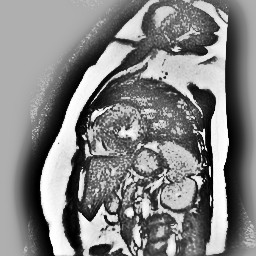
\includegraphics[width=0.19\textwidth]{./data/failures/HCMNet_2000062/00_SAX/9/9.png} &
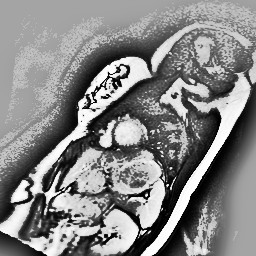
\includegraphics[width=0.19\textwidth]{./data/failures/HCMNet_2400044/00_SAX/2/5.png} &
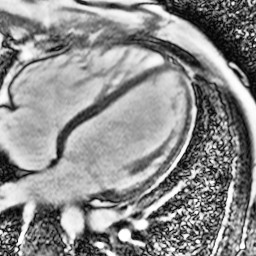
\includegraphics[width=0.19\textwidth]{./data/failures/HCMNet_2600079/01_HLA/00/0.png} &
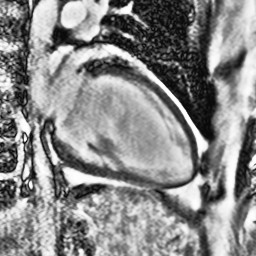
\includegraphics[width=0.19\textwidth]{./data/failures/HCMNet_2600079/02_VLA/00/0.png} \\

\multicolumn{4}{c}{结构定位} \\

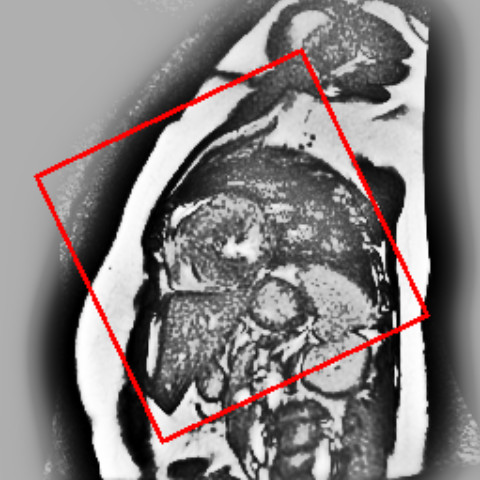
\includegraphics[width=0.19\textwidth]{./data/failures/HCMNet_2000062/00_SAX/9/9_bbox.png} &
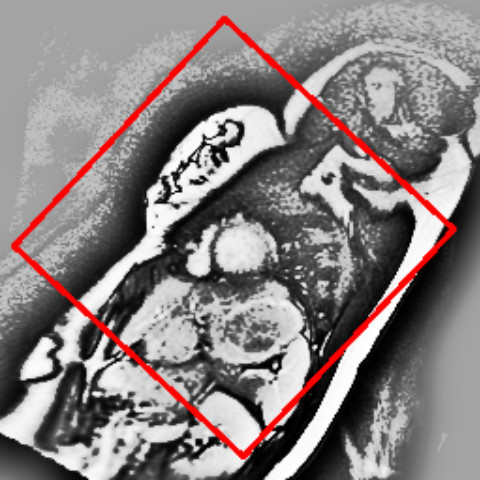
\includegraphics[width=0.19\textwidth]{./data/failures/HCMNet_2400044/00_SAX/2/5_bbox.png} &
\includegraphics[width=0.19\textwidth]{./data/failures/HCMNet_2600079/01_HLA/00/0_bbox.png} &
\includegraphics[width=0.19\textwidth]{./data/failures/HCMNet_2600079/02_VLA/00/0_bbox.png} \\

\multicolumn{4}{c}{在典型方向下的分割预测值:$S^\prime$} \\

\includegraphics[width=0.19\textwidth]{./data/failures/HCMNet_2000062/00_SAX/9/9_pred.png} &
\includegraphics[width=0.19\textwidth]{./data/failures/HCMNet_2400044/00_SAX/2/5_pred.png} &
\includegraphics[width=0.19\textwidth]{./data/failures/HCMNet_2600079/01_HLA/00/0_pred.png} &
\includegraphics[width=0.19\textwidth]{./data/failures/HCMNet_2600079/02_VLA/00/0_pred.png} \\
\bottomrule

\multicolumn{4}{c}{在典型方向下的分割真实值:$\hat{S}^\prime$} \\

\includegraphics[width=0.19\textwidth]{./data/failures/HCMNet_2000062/00_SAX/9/9_gt.png} &
\includegraphics[width=0.19\textwidth]{./data/failures/HCMNet_2400044/00_SAX/2/5_gt.png} &
\includegraphics[width=0.19\textwidth]{./data/failures/HCMNet_2600079/01_HLA/00/0_gt.png} &
\includegraphics[width=0.19\textwidth]{./data/failures/HCMNet_2600079/02_VLA/00/0_gt.png} \\
\bottomrule

\end{tabular}

\caption[\captiontitle]{\captiontitle{}.详细讨论参考正文.}
\label{fig:failure}
\end{center}
\end{figure*}


我们也观察到偶然分割失败的例子,其中一些例子如图 \ref{fig:failure} 所示.
每一个失败的例子都有一两个可以解释的原因.
最左一栏的例子为一个严重心肌肥大的病人的 \SA{} 切面.
这样的例子是数据集中比较罕见的,所以导致网络分割结果很差.
第二栏的例子是另一个病人的 \SA{} 切面,其右室被错误的分割.
这个图中的灰度整体比较低,导致经过直方图均衡处理之后对比度太高.
第三和第四栏的图中扫描分辨率太高,以致于心脏占了整个图的大部分区域,进而导致缺少上下文信息.
这里例子中的糟糕分割结果都是由于图像没能正确地变换到一个典型方向.
然而,需要强调的是,这些事后诸葛亮的分析;我们并不能直接给出这些特征与分割失败之间的关系.

\subsection{2017 MICCAI \miccaidata{} 数据集}
\renewcommand{\captiontitle}{在 2017 MICCIA \miccaidata{} 数据集上的分割准确率}
\begin{table*}
\hl{
\begin{center}
\begin{tabular}{lccc} \hline
\toprule
结构           & 左室血池 & 右室血池 & 左室心肌 \\
\midrule
\multicolumn{4}{c}{Jaccard 系数(\IoU{})} \\
\midrule
\omeganet{}         & \textbf{\ACDCONJLVBP{}}  & \textbf{\ACDCONJRVBP{}}  & \ACDCONJLVMY{}           \\
\citet{Isensee2018} & \ACDCFINJLVBP{}          & \ACDCFINJRVBP{}          & \textbf{\ACDCFINJLVMY{}} \\
\citet{Isensee2017} & \ACDCFIOJLVBP{}          & \ACDCFIOJRVBP{}          & \ACDCFIOJLVMY{}          \\
\midrule
\multicolumn{4}{c}{Dice 系数} \\
\midrule
\omeganet{}         & \textbf{\ACDCONDLVBP{}}  & \textbf{\ACDCONDRVBP{}}  & \ACDCONDLVMY{}           \\
\citet{Isensee2018} & \ACDCFINDLVBP{}          & \ACDCFINDRVBP{}          & \textbf{\ACDCFINDLVMY{}} \\
\citet{Isensee2017} & \ACDCFIODLVBP{}          & \ACDCFIODRVBP{}          & \ACDCFIODLVMY{}          \\
\bottomrule
\end{tabular}
\caption[\captiontitle{}]{
\hl{
\captiontitle{}.
\miccaidata{} 挑战的分割准确率用 Dice 系数计算,其他的地方使用 \IoU{} 计算;因此这里把两个都计算出来了.
(提示,$\mathrm{Dice} = 2 * \mathrm{\IoU{}} / (1 + \mathrm{\IoU{}})$)
我们给出了 \omeganet{} 网络 B 的结果;\citet{Isensee2017} 发表在 STACOM 上的结果;以及 \citet{Isensee2018} 在 \url{arxiv.org} 上预发表的结果.
每一前景类别的最佳结果用加粗字体标出.
}
}
\label{tab:acdc}
\end{center}
}
\end{table*}

\citet{Isensee2017} 在 \miccaidata{} 排行榜上取得了最佳的成绩;他们 \citep{Isensee2018} 还预发表 \footnote{https://arxiv.org/abs/1707.00587v2} 了一个更好的结果.
为了与他们的结果比较,我们在 MICCAI \miccaidata{} 上从头开始训练了 \omeganet{} 网络 B,使用五折交叉验证,并且每一个受试者的数据仅出现在其中一折中.
\omeganet{} 模型,\citet{Isensee2017} 以及 \citet{Isensee2018} 的分割准确率对比如表 \ref{tab:acdc} 所示.
相比于 \citet{Isensee2017},我们的结果中每一类的 \IoU{} 都更高:左室血池($\ACDCONJLVBP{}$ vs $\ACDCFIOJLVBP{}$),右室血池($\ACDCONJRVBP{}$ vs $\ACDCFIOJRVBP{}$)和左室心肌($\ACDCONJLVMY{}$ vs $\ACDCFIOJLVMY{}$).
相比于 \citet{Isensee2018},我们的左室血池($\ACDCONJLVBP{}$ vs $\ACDCFINJLVBP{}$)和右室血池($\ACDCONJRVBP{}$ vs $\ACDCFINJRVBP{}$)的 \IoU{} 更高,但是左室心肌($\ACDCONJLVMY{}$ vs $\ACDCFINJLVMY{}$)的较低.
